%\documentclass[letterpaper,12pt]{report}
%\usepackage[spanish]{babel}
%\usepackage{graphicx, color}
%\usepackage{amsmath}
%\usepackage{amscd}
%\usepackage{youngtab}
%\usepackage{titlesec}
%\usepackage[latin1]{inputenc}
%\usepackage{listings}
%\usepackage{multicol}
%\usepackage{enumerate}
%\usepackage{amssymb}
%\usepackage{amsthm}
%\usepackage{syntonly}
%\usepackage{fancyhdr}
%\usepackage{hyperref}
%\begin{document}
\section{Decaimiento $A_{k}\rightarrow B_{j}\bar{C}_{i}$}
%****************figuras Higgs�s decay****************************************
\begin{figure}[h]
\begin{center}
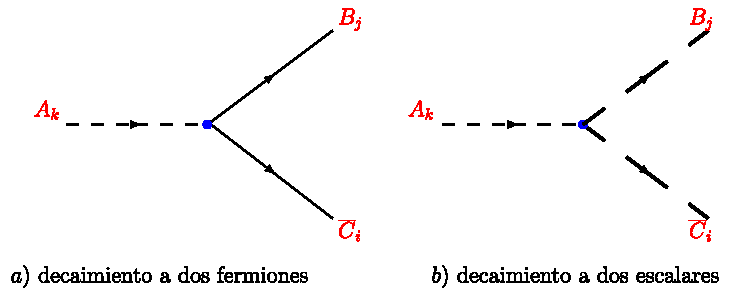
\includegraphics[scale=0.8]{DecaiABC1}
\caption{Decaimiento a dos cuerpos}
\label{Decaimiento a dos
cuerpos}
\end{center}
\end{figure}
%*****************************************************************************
Consideremos la siguiente lagrangiana asociada al proceso de
decaimiento general de una part�cula a dos nuevas part�culas, fig.
\ref{Decaimiento a dos cuerpos}:
%-------------------------------
\begin{equation}
\mathcal{L}=g\overline{C}_{i}(O_{Lijk}P_{L}+O_{Rijk}P_{R})B_{j}A_{k}
\label{lagrangiana dos cuerpos}
\end{equation}
%-------------------------------
Los t�rminos $O_{Lijk}$ y $O_{Rijk}$ son los respectivos acoples de
las tres part�culas involucradas en el proceso.  $P_{L}$ y $P_{R}$
son en general los proyectores, los cuales son determinados por las
siguiente expresi�n:
%------------------------------------
\begin{equation}
P_{L}=\frac{1-\gamma^{5}}{2} \hspace{0.5cm};\hspace{0.5cm}
P_{R}=\frac{1+\gamma^{5}}{2}. \label{proyectors}
\end{equation}
%------------------------------------
Para calcular la \emph{tasa de decaimiento}, usamos la siguiente
expresi�n \cite{Peskin,Griffiths}:
%-------------------------------
\begin{equation*}
\frac{d\Gamma}{d\Omega_{cm}}=\frac{|\overrightarrow{P}_{1}|}{32\pi^{2}m_{A}^{2}}
\sum_{S_{B}S_{C}} |\mathcal{M}(A\longrightarrow B+C)|^{2}
\end{equation*}
%-------------------------------
%-------------TASA DE DECAIMINETO-------------------
\begin{equation}
\Rightarrow\Gamma=\frac{|\overrightarrow{P}_{1}|}{16\pi
m_{A}^{2}}\sum_{s_{1}s_{2}} |\mathcal{M}(A\longrightarrow
B(p_{1},s_{1})+C(p_{2},s_{2})|^{2}, \label{tasa de decaimiento}
\end{equation}
%---------------------------------------------------
donde la suma es tomada sobre los estados de polarizaci�n de los
espines de las dos part�culas finales.
%********************figuras Higgs�s decay con reglas de Feynman*************
\begin{figure}[h]
\begin{center}
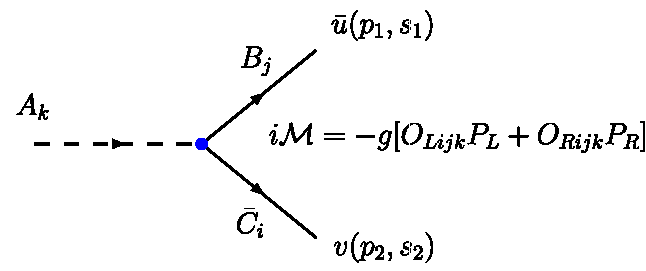
\includegraphics[scale=0.8]{ReglasFdoscuerpos}
\caption{reglas de Feynman}
\label{Decaimiento (reglas de Feynman)}
\end{center}
\end{figure}
%****************************************************************************
Las correspondientes reglas de Feynman son mostradas en la fig.
\ref{Decaimiento (reglas de Feynman)}. En �sta se muestra como le
son asociado las cantidades correspondientes tanto al v�rtice como a
las patas externas.
\section{Amplitud invariante de transici�n para el decaimiento
$A_{k}\rightarrow B_{j}\bar{C}_{i}$}
La \emph{Amplitud invariante de transici�n} es determinada por el
producto de todas las cantidades que contribuyen al diagrama, es
decir,
%*************AMPLITUD****************************
\begin{align}
i\mathcal{M}&=-g\overline{u}(p_{1}s_{1})[O_{Lijk}P_{L}+O_{Rijk}P_{R}]v(p_{2}s_{2})\nonumber\\
&=-g[O_{Lijk}\overline{u}(p_{1}s_{1})P_{L}v(p_{2}s_{2})+
O_{Rijk}\overline{u}(p_{1}s_{1})P_{R}v(p_{2}s_{2})],
\label{amplitud}
\end{align}
%*************************************************
donde $\overline{u}(p s)$ y $v (p s)$ son las respectivas espinores
asociados a la expansi�n de Fourier del campo de Dirac.

As�, tenemos:
%**********************************************
\begin{align}
|\mathcal{M}|^{2}=g^{2}&[O_{Lijk}\overline{u}(p_{1}s_{1})P_{L}v(p_{2}s_{2})+
O_{Rijk}\overline{u}(p_{1}s_{1})P_{R}v(p_{2}s_{2})]^{\dagger}\nonumber\\
&[O_{Lijk}\overline{u}(p_{1}s_{1})P_{L}v(p_{2}s_{2})+
O_{Rijk}\overline{u}(p_{1}s_{1})P_{R}v(p_{2}s_{2})].
\end{align}
%**********************************************
Para calcular el cuadrado de la amplitud invariante de transici�n,
debemos tomar en cuenta las siguientes propiedades asociadas a los
espinores y a las matrices de Dirac:
%*******************PROPIEDADES***************************
\begin{align}
\overline{u}(p_{1}s_{1})=&u(p_{1}s_{1})^{\dagger}\gamma^{0}\nonumber\\
\overline{v}(p_{1}s_{1})=&v(p_{1}s_{1})^{\dagger}\gamma^{0}\\
\{\gamma^{\mu},\gamma^{\nu}\}=&2g^{\mu\nu},\{\gamma^{0},\gamma^{5}\}=0\\
tr[\gamma^{\mu}]=&0,\hspace{0.2cm}tr[\gamma^{\mu}\gamma^{\nu}]=4g^{\mu\nu}
\label{suma de trazas}\\
(P_{L})^{2}=P_{L},\hspace{0.2cm}(P_{R})^{2}=&P_{R},\hspace{0.2cm}P_{L}P_{R}=0
\label{propiedades de proyectores}\\
\gamma^{\mu}P_{L}=&P_{R}\gamma^{\mu}
\label{intercambio gama con proyector}\\
[\overline{u}(p_{1}s_{1})v(p_{2}s_{2})]^{\dagger}=&
\overline{v}(p_{2}s_{2})u(p_{1}s_{1})\\
[\overline{u}(p_{1}s_{1})P_{L}v(p_{2}s_{2})]^{\dagger}=&
\overline{v}(p_{2}s_{2})P_{R}u(p_{1}s_{1})
\label{UyVconproyectores}\\
\sum_{s_{1}}u(p_{1}s_{1})\overline{u}(p_{1}s_{1})=&(p_{\mu}\gamma^{\mu}+m)\nonumber\\
\sum_{s_{1}}v(p_{1}s_{1})\overline{v}(p_{1}s_{1})=&(p_{\mu}\gamma^{\mu}-m),
\label{UUbarraVVbarra}
\end{align}
%********************************************************
as�, usando la ecuaci�n (\ref{UyVconproyectores}) tenemos que:
%***************************************************
\begin{align}
\sum_{s_{1},s_{2}}|\mathcal{M}|^{2}=
\sum_{s_{1},s_{2}}g^{2}&[O_{L}\overline{u}(p_{1}s_{1})P_{L}v(p_{2}s_{2})+
O_{R}\overline{u}(p_{1}s_{1})P_{R}v(p_{2}s_{2})]^{\dagger}\nonumber\\
&[O_{L}\overline{u}(p_{1}s_{1})P_{L}v(p_{2}s_{2})+
O_{R}\overline{u}(p_{1}s_{1})P_{R}v(p_{2}s_{2})]\nonumber\\
=\sum_{s_{1},s_{2}}g^{2}&[O_{L}^{*}\overline{v}(p_{2}s_{2})P_{R}u(p_{1}s_{1})+
O_{R}^{*}\overline{v}(p_{2}s_{2})P_{L}u(p_{1}s_{1})]\nonumber\\
&[O_{L}\overline{u}(p_{1}s_{1})P_{L}v(p_{2}s_{2})+
O_{R}\overline{u}(p_{1}s_{1})P_{R}v(p_{2}s_{2})]\nonumber
\end{align}
%***************************************************
%************************SUMATORIAS***********************
\begin{align}
\Rightarrow\sum_{s_{1},s_{2}}|\mathcal{M}|^{2}=
&g^{2}\Big[\sum_{s_{1},s_{2}}(O_{L})^{2}\overline{v}(p_{2}s_{2})P_{R}u(p_{1}s_{1})
\overline{u}(p_{1}s_{1})P_{L}v(p_{2}s_{2})\nonumber\\
+&\sum_{s_{1},s_{2}}(O_{R})^{2}\overline{v}(p_{2}s_{2})P_{L}u(p_{1}s_{1})
\overline{u}(p_{1}s_{1})P_{R}v(p_{2}s_{2})\nonumber\\
+&\sum_{s_{1},s_{2}}O_{L}^{*}O_{R}\overline{v}(p_{2}s_{2})P_{R}u(p_{1}s_{1})
\overline{u}(p_{1}s_{1})P_{R}v(p_{2}s_{2})\nonumber\\
+&\sum_{s_{1},s_{2}}O_{R}^{*}O_{L}\overline{v}(p_{2}s_{2})P_{L}u(p_{1}s_{1})
\overline{u}(p_{1}s_{1})P_{L}v(p_{2}s_{2})\Big]. \label{sumatorias}
\end{align}
%*********************************************************
Cada una de las sumatorias involucradas en la ec. (\ref{sumatorias})
debe calcularse por separado. En cada una de ellas deben expresarse
los productos espinoriales en t�rminos de sus componentes. Por
ejemplo para la primera sumatoria tenemos:
%------------------------------
\begin{align}
&\sum_{s_{1},s_{2}}[\overline{v}(p_{2}s_{2})P_{R}u(p_{1}s_{1})]
[\overline{u}(p_{1}s_{1})P_{L}v(p_{2}s_{2})]\nonumber\\
=&\sum_{s_{1},s_{2}}
\overline{v}_{\alpha}(p_{2}s_{2})P_{R\alpha\beta}u_{\beta}(p_{1}s_{1})
\overline{u}_{\theta}(p_{1}s_{1})P_{L\theta\rho}v_{\rho}(p_{2}s_{2})\nonumber\\
=&\Big[\sum_{s_{1}}u_{\beta}(p_{1}s_{1})\overline{u}_{\theta}(p_{1}s_{1})P_{L\theta\rho}\Big]
\Big[\sum_{s_{2}}v_{\rho}(p_{2}s_{2})\overline{v}_{\alpha}(p_{2}s_{2})P_{R\alpha\beta}\Big].
\end{align}
%------------------------------
Usando la propiedad (\ref{UUbarraVVbarra}) tenemos:
%------------------------------
\begin{align}
=&(p_{1\mu}\gamma^{\mu}+m_{p_{1}})_{\beta\theta}P_{L\theta\rho}
(p_{2\nu}\gamma^{\nu}-m_{p_{2}})_{\rho\alpha}P_{R\alpha\beta}\nonumber\\
=&\operatorname{tr}[(p_{1\mu}\gamma^{\mu}+m_{p_{1}})P_{L}
(p_{2\nu}\gamma^{\nu}-m_{p_{2}})P_{R}]\nonumber\\
=&\operatorname{tr}[P_{R}(p_{1\mu}\gamma^{\mu}+m_{p_{1}})P_{L}
(p_{2\nu}\gamma^{\nu}-m_{p_{2}})]\nonumber\\
=&\{p_{1\mu}p_{2\nu}\operatorname{tr}[P_{R}\gamma^{\mu}P_{L}\gamma^{\nu}]
-p_{1\mu}m_{2}\operatorname{tr}[P_{R}\gamma^{\mu}P_{L}]
+m_{1}p_{2\nu}\operatorname{tr}[P_{R}P_{L}\gamma^{\nu}]\nonumber\\
&-m_{1}m_{2}\operatorname{tr}[P_{R}P_{L}]\},
\end{align}
%------------------------------
usando la propiedad c�clica de la traza y las ecuaciones (\ref{suma
de trazas}), (\ref{propiedades de proyectores}), (\ref{intercambio
gama con proyector}), tenemos:
%------------------------------
\begin{align}
&=\{p_{1\mu}p_{2\nu}\operatorname{tr}[\gamma^{\mu}P_{L}P_{L}\gamma^{\nu}]
\}=p_{1\mu}p_{2\nu}\operatorname{tr}[\gamma^{\mu}P_{L}\gamma^{\nu}]\nonumber\\
&=p_{1\mu}p_{2\nu}\operatorname{tr}[\gamma^{\mu}(\frac{1-\gamma^{5}}{2})\gamma^{\nu}]
=\frac{1}{2}p_{1\mu}p_{2\nu}\{[\gamma^{\mu}\gamma^{\nu}]-[\gamma^{\mu}\gamma^{5}\gamma^{\nu}]\}\nonumber\\
&=2p_{1\mu}p_{2\nu}g^{\mu\nu}=2p_{1\mu}p_{2}^{\nu}\nonumber\\
&=2(E_{1}E_{2}-\vec{p}_{1}\cdot\vec{p}_{2}),
\end{align}
%------------------------------
donde $E_{1}$, $E_{2}$, $\vec{p}_{1}$, $\vec{p}_{2}$, son las
energ�as y los momentos correspondientes a las part�culas
$A(p_{1}s_{1})$ y $B(p_{2}s_{2})$ involucradas en el proceso. Adem�s
debido a la \emph{conservaci�n de momento}
$\vec{p}_{1}=-\vec{p}_{2}$, as� tenemos:
%------------------------------
\begin{align}
\sum_{s_{1},s_{2}}\overline{v}(p_{2}s_{2})P_{R}u(p_{1}s_{1})
\overline{u}(p_{1}s_{1})P_{L}v(p_{2}s_{2})=2(E_{1}E_{2}+|{\vec{p}}_{1}|^{2}).
\label{suma0}
\end{align}
%------------------------------
Igualmente, debido a la conservaci�n de energ�a tenemos que:
%------------------------------
\begin{align}
m_{A}=E_{1}+E_{2} \Rightarrow
E_{1}E_{2}=\frac{m_{A}^{2}-E_{1}^{2}-E_{2}^{2}}{2}, \label{cons. de
energia}
\end{align}
%------------------------------
y de la conservaci�n de momento:
%------------------------------
\begin{align}
|{\vec{p}}_{1}|^{2}&=|{\vec{p}}_{2}|^{2},\nonumber\\
E_{1}^{2}-m_{1}^{2}&=E_{2}^{2}-m_{2}^{2} \Rightarrow
(\frac{E_{1}^{2}-E_{2}^{2}}{2})=(\frac{m_{1}^{2}-m_{2}^{2}}{2}).
\label{cons. de momento}
\end{align}
%------------------------------
Reemplazando las ecs. (\ref{cons. de energia}) y (\ref{cons. de
momento}) en la ec. (\ref{suma0}), obtenemos finalmente que:
%------------------------------------------
\begin{align}
\sum_{s_{1},s_{2}}\overline{v}(p_{2}s_{2})P_{R}u(p_{1}s_{1})
\overline{u}(p_{1}s_{1})P_{L}v(p_{2}s_{2})=(m^{2}_{A}-m^{2}_{1}-m^{2}_{2}).
\label{suma1}
\end{align}
%------------------------------------------
Mediante un procedimiento totalmente an�logo, se demuestra que:
%-------------------------
\begin{equation}
\sum_{s_{1},s_{2}}\overline{v}(p_{2}s_{2})P_{L}u(p_{1}s_{1})
\overline{u}(p_{1}s_{1})P_{R}v(p_{2}s_{2})=(m^{2}_{A}-m^{2}_{1}-m^{2}_{2}),
\label{suma2}
\end{equation}
\begin{equation}
\sum_{s_{1},s_{2}}\overline{v}(p_{2}s_{2})P_{R}u(p_{1}s_{1})
\overline{u}(p_{1}s_{1})P_{R}v(p_{2}s_{2})=-2m_{1}m_{2},
\label{suma3}
\end{equation}
\begin{equation}
\sum_{s_{1},s_{2}}\overline{v}(p_{2}s_{2})P_{L}u(p_{1}s_{1})
\overline{u}(p_{1}s_{1})P_{L}v(p_{2}s_{2})=-2m_{1}m_{2}.
\label{suma4}
\end{equation}
%-------------------------
Reemplazando las ecs. (\ref{suma1})\ldots(\ref{suma4}) en la ec.
(\ref{sumatorias}), obtenemos finalmente que:
%-------------------------
\begin{align}
\sum_{s_{1},s_{2}}|\mathcal{M}|^{2}=g^{2}&\Big\{[(O_{Lijk})^{2}
+(O_{Rijk})^{2}](m^{2}_{A}-m^{2}_{1}-m^{2}_{2})\nonumber\\
&-2m_{1}m_{2}[O_{Lijk}^{*}O_{Rijk} +O_{Rijk}^{*}O_{Lijk}]\Big\}.
\label{amplitudcuadrada}
\end{align}
%-------------------------
Ya calculada la expresi�n anterior tan s�lo nos falta calcular
$|\vec{p_{1}}|^{2}$, para as� de este modo determinar la tasa de
decaimiento (\ref{tasa de decaimiento}).
\section{Momento final en el decaimiento
$A_{k}\rightarrow B_{j}\bar{C}_{i}$} Sabemos de la conservaci�n de
momento y de la energ�a que:
%-------------------------
\begin{align}
|\vec{p_{1}}|^{2}=&|\vec{p_{2}}|^{2}=E^{2}_{2}-m_{2}^{2}=(E_{A}-E_{1})^{2}-m_{2}^{2}\nonumber\\
=&E_{A}^{2}-2E_{A}E_{1}+(E_{1}^{2})-m_{2}^{2}\nonumber\\
=&E_{A}^{2}-2E_{A}E_{1}+(|\vec{p_{1}}|^{2}+m_{1}^{2})-m_{2}^{2},
\label{|p1|}\nonumber
\end{align}
%-------------------------
y as�:
%-------------------------
\begin{align}
E_{1}&=\frac{1}{2E_{A}}(E_{A}^{2}+m_{1}^{2}-m_{2}^{2})\nonumber\\
\Rightarrow |\vec{p_{1}}|^{2}+m_{1}^{2}
&=\frac{1}{4E_{A}^{2}}(E_{A}^{2}+m_{1}^{2}-m_{2}^{2})^{2}.\nonumber
\end{align}
%-------------------------
En el sistema en reposo de la part�cula $A$, tenemos que
$E_{A}=m_{A}$, y as�:
%------------------------------
\begin{align}
|\vec{p_{1}}|=
\frac{1}{2m_{A}}\Big[(m_{A}^{2}-m_{2}^{2}+m_{1}^{2})^{2}-4m_{A}^{2}m_{1}^{2}\Big]^{1/2}.
\end{align}
%------------------------------
Ahora, definiendo la funci�n:
%------------------------------
\begin{align}
\boxed{\lambda(a,b,c)=(a-b+c)^{2}-4ac}, \label{funcionlanda}
\end{align}
%------------------------------
tenemos finalmente que:
%------------------------------
\begin{align}
|\vec{p}_{1}|=\frac{1}{2m_{A}}\lambda^{1/2}(m_{A}^{2},m_{2}^{2},m_{1}^{2}).
\label{p1}
\end{align}
%------------------------------
\section{Tasa de Decaimiento
$A_{k}\rightarrow B_{j}\bar{C}_{i}$} Reemplazando las ecs.
(\ref{amplitudcuadrada}) y (\ref{p1}), obtenemos que la \emph{tasa
de decaimiento} ec. (\ref{tasa de decaimiento}) est� dada por:
%****************TASA DE DECAIMINETO***********************
\begin{align}
\Gamma(A_{k}\rightarrow B_{j}\bar{C}_{i})=
g^{2}\frac{\lambda^{1/2}(m_{A}^{2},m_{2}^{2},m_{1}^{2})}{16\pi
m_{A}^{3}}&\Big\{[(O_{Lijk})^{2}+(O_{Rijk})^{2}](m^{2}_{A}-m^{2}_{1}-m^{2}_{2})\nonumber\\
&-2m_{1}m_{2}[O_{Lijk}^{*}O_{Rijk} +O_{Rijk}^{*}O_{Lijk}]\Big\}.
\label{tasa de decaimiento final}
\end{align}
%**********************************************************
%\end{document}
